% Template for ICASSP-2018 paper; to be used with:
%          spconf.sty  - ICASSP/ICIP LaTeX style file, and
%          IEEEbib.bst - IEEE bibliography style file.
% --------------------------------------------------------------------------
\documentclass{article}
\usepackage{spconf,amsmath,amssymb,graphicx,bm}
\graphicspath{{figures/}}

\newcommand{\R}{\mathbb{R}}
\renewcommand{\vec}[1]{\ensuremath{\mathbf{#1}}}
\providecommand{\mat}[1]{\ensuremath{\mathbf{#1}}}
\providecommand{\vx}{\vec{x}}
\providecommand{\vy}{\vec{y}}
\providecommand{\vw}{\vec{w}}
\providecommand{\vu}{\vec{u}}
\providecommand{\vA}{\vec{A}}
\providecommand{\vD}{\vec{D}}
\providecommand{\norm}[1]{\left\lVert#1\right\rVert}
\DeclareMathOperator*{\argmin}{arg\,min}
\DeclareMathOperator*{\argmax}{arg\,max}

\title{Optimal Measurement Configuration in \\ Computational Multispectral Imaging With a Diffractive Lens}

\name{Evan Widloski \qquad Ulas Kamaci \qquad Farzad Kamalabadi}
\address{
Department of Electrical and Computer Engineering and Coordinated Science Laboratory, \\
University of Illinois at Urbana-Champaign, Urbana, IL 61801, USA
}

\begin{document}
\maketitle

\begin{abstract}
% Spectral imaging, forming images of a scene at many wavelengths, is a
% fundamental analysis technique with many scientific applications. Diffractive
% lenses can achieve very high resolution in x-ray and UV regimes as compared to
% reflective and refractive optics. Their wavelength dependent focal length
% enables them to be used in spectral imaging of polychromatic sources, where the
% focused image of each spectral component is formed at different distances from
% the diffractive lens. If measurements are taken at each of these focus
% locations, it is possible to computationally reconstruct the spectral scene by
% solving an inverse problem. In this paper, we propose a greedy algorithm for
% finding a measurement configuration which results in better reconstructions than
% a conventional configuration selection strategy.

In this paper, we investigate the problem of data acquisition in a multispectral
diffractive imaging system.  Diffractive systems have the property that the
spectral components of a polychromatic source are focused at different distances
from the lens.  This means that in order to image a source at more than one
wavelength, multiple measurements must be made with a moving detector. However,
the choice of where to make these measurements is non-obvious and has
implications on the quality of the reconstructions. Furthermore, an exhaustive
search of all possible measurement configurations grows exponentially with the
number of sources and is computationally infeasible. We propose a greedy
backward elimination algorithm
\end{abstract}

\begin{keywords}
Spectral imaging, diffractive optics, measurement configuration, sequential
backward selection, subset selection
\end{keywords}

\section{Introduction}
\label{sec:intro}
Spectral imaging is the formation of images at different wavelengths in the
electromagnetic spectrum.  With images usually taken in the visible, x-ray,
ultraviolet (UV), or infrared bands (IR), it has applications in medicine, geographic
surveying, astronomy, and solar physics.  Spectral imaging can be further broken
down into the categories of \emph{hyperspectral imaging} and \emph{multispectral imaging}.
Hyperspectral imaging is the capture of a scene over a contiguous spectrum,
while multispectral imaging is the capture of a set narrow, usually non-adjacent
bands of interest.  In both cases, a polychromatic source must be first
separated into its spectral components before being captured.  There are a
number of ways to achieve this, but a common method is to use a set of
configurable optical filters.  For example, the spectral imager on the Solar
Dynamics Observatory uses a rotating drum of optical filters to selectively pass
light of specific wavelengths of interest.

% Spectral imaging is forming images of a scene as a function of wavelength, is a
% fundamental diagnostic technique in various fields such as astronomy,
% surveillance, agriculture and medicine \cite{shaw2003spectral},
% \cite{garini2006spectral}. Forming a three dimensional (3D) data-cube (one
% wavelength and two spatial dimensions) with two dimensional (2D) detector
% measurements can be done by taking multiple exposures. To capture the spectrum
% of a scene, conventional spectral imagers combine regular camera optics with
% either additional wavelength filters or dispersive elements (e.g diffraction
% grating).

An alternative approach is to use a diffractive lens to perform spectral
imaging.  Diffractive lenses have the property that light at different
wavelengths will exit the lens at different angles, which has the effect of
creating a focused image of the light source at separate planes for each
spectral component of the source (Figure \ref{fig:diff_lens}(a)).

Diffractive lenses are often preferred in the UV or x-ray regimes over
reflective optics because manufacturing tolerances at these wavelengths must be
much tighter than in the visible regime in order to get a similar optical
performance.  Since diffractive optics can be manufactured using a
photolithographic process they can be produced at a higher precision than
the grinding process used to produce conventional reflective optics.
Similarly, refractive optics are unsuitable for UV or x-ray imaging because
glass is opaque at these wavelengths. Figures \ref{fig:diff_lens}(b) and
\ref{fig:diff_lens}(c) are two examples of a pattern that can be etched into
silicon wafer to produce a diffractive lens.

\begin{figure}[htb]

\begin{minipage}[b]{0.48\linewidth}
  \centering
  \centerline{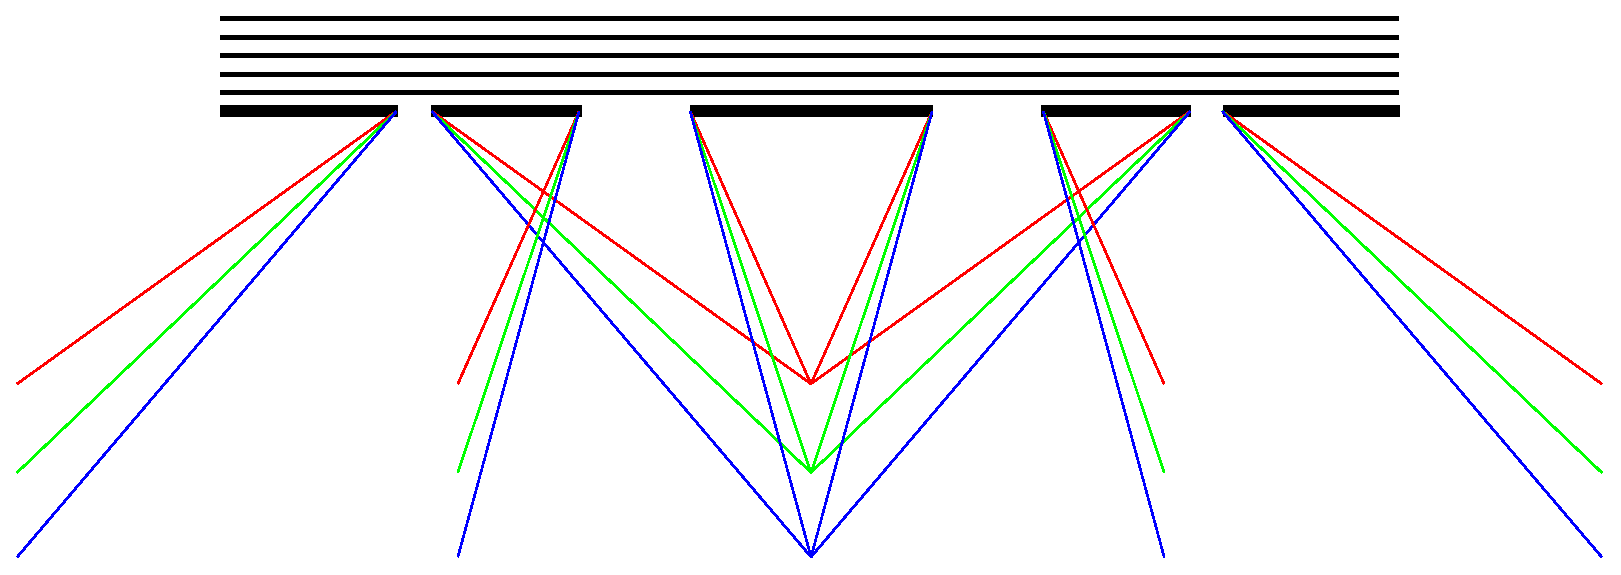
\includegraphics[width=4.0cm]{diffraction_ps_rgb}}
  \centerline{(a)}\medskip
\end{minipage}
\hfill
\begin{minipage}[b]{0.24\linewidth}
  \centering
  \centerline{\includegraphics[width=2.0cm]{zoneplate}}
  \centerline{(b)}\medskip
\end{minipage}
\hfill
\begin{minipage}[b]{0.24\linewidth}
  \centering
  \centerline{\includegraphics[width=2.0cm]{photonsieve}}
%  \vspace{1.5cm}
  \centerline{(c)}\medskip
\end{minipage}
\caption{(a) diffraction of a polychromatic wave through a diffractive lens (b) Fresnel zone
plate (c) photon sieve}
\label{fig:diff_lens}
%
\end{figure}

While diffraction produces a focused image of each source at separate planes, it
.  This means that each measurement is actually a sum of all spectral
components of the source at varying degrees of focus.  An inverse problem
consisting of disentangling and deblurring of measurements must be solved in
order to recover the original source components.  Traditionally, measurement
locations are selected at the plane of focus for each spectral component.
However, as we show later in this paper, it is possible to improve on the
reconstruction quality in some situations by making measurements away from these
focal positions. We propose a greedy backward selection algorithm for
automatically discovering such a measurement configuration. Additionally, we
provide some bounds under which the greedy algorithm outperforms the traditional
selection approach.

% A different approach is to use a diffractive lens to perform spectral imaging.
% Diffractive lenses focus light using the diffraction principle. They have
% wavelength dependent focal length which is the property that enables them to be
% used as spectral imagers (see Figure \ref{fig:diff_lens}). Examples of
% diffractive lenses are Fresnel zone plates and their modifications (e.g. photon
% sieve) (see Figure \ref{fig:diff_lens}). Diffractive lenses are preferred in
% applications in UV and x-ray regimes where they can provide high resolution
% whereas reflective optics are very costly to manufacture to achieve high
% resolution and refractive lenses cannot be used due to light absorption in these
% regimes.


% Photon sieve spectral imaging (PSSI) is a modality that takes the advantage of
% the wavelength dependent focal length of a photon sieve to perform high
% resolution spectral imaging \cite{oktem2014icip}. It takes multiple exposures of
% the scene at different distances from the lens. Figure \ref{fig:pssi_drawing}
% illustrates the PSSI measurements for a scene radiating at two wavelengths
% $\lambda_1$ and $\lambda_2$. Each measurement consists of blurred superposition
% of the spectral images. The spectral images are then reconstructed from these
% measurements by solving a multi-frame deconvolution problem.


\begin{figure}[htb]
  \begin{minipage}[b]{1\linewidth}
    \centering
    \centerline{\includegraphics[width=8.5cm]{drawing}}
  \end{minipage}
  \caption{Imaging a scene with emissions at wavelengths $\lambda_1$ and
  $\lambda_2$. Measurements $y_1$ and $y_2$ are taken at two positions where one wavelength
  is in focus and the other is out of focus.}
  \label{fig:pssi_drawing}
\end{figure}

% Choice of measurement planes is an important factor affecting the reconstruction
% quality of the spectral images. Where to take measurements to maximize the
% fidelity of the reconstructions?

% One way is to scan the
% wavelength dimension by using color filters with narrow bandpass to filter
% desired wavelengths at each exposure. Another way is to capture the whole
% spectrum of a portion of the scene at an exposure, and scan a spatial dimension.
% In both methods, the 3D data-cube is then simply reconstructed by stacking the
% 2D measurements in the scanning dimension.

% There are also computational methods which rely on signal processing methods and
% computational power to improve upon the conventional methods in terms of spatial
% and spectral resolutions, total exposure time etc. They utilize more
% sophisticated image acquisition techniques than the conventional scanning-based
% methods, and computationally reconstruct the data-cube from multiplexed/encoded
% measurements. Such methods include compressive coded aperture snapshot spectral
% imaging (CASSI) [REF], compressive hyperspectral imaging by separable spectral
% and spatial operators (CHISS) [REF], and photon sieve spectral imaging (PSSI)
% \cite{oktem2014icip}.

% We will use PSSI as an example modality to explain and demonstrate our work
% because it  uses a diffractive lens, and it is a computational spectral imaging
% modality \cite{oktem2014icip}. Photon sieves, just like Fresnel zone plates, are
% diffractive lenses that use diffraction phenomenon to focus light. Diffractive
% lenses are preferred in applications in UV and x-ray regimes since they can
% provide high resolution whereas reflective optics are very costly to manufacture
% to achieve high resolution and refractive lenses cannot be used due to light
% absorption. They have wavelength dependent focal length which is what behind the
% working principle of PSSI. It takes multiple exposures at different distances
% from the lens to sample the measurement space.

\section{Forward Model}
\label{sec:format}
In this section, we mathematically model a multispectral diffractive imaging
system. Consider a polychromatic source that has $S$ two-dimensional spectral
components $\bm{x}_1, \dots, \bm{x}_S$. Using a moving detector, we make $M$
two-dimensional measurements $\bm{y}_1, \dots, \bm{y}_M$ at different distances
from the lens. Due to linearity, each measurement is a superposition of blurred
versions of the $S$ sources.  More formally,

$$
\bm{y}_m = \sum_{s=1}^S \bm{h}_{m,s} \ast \bm{x}_s
$$

where $\bm{h}_{m,s}$ is a blurring kernel known as a \emph{point spread
  function} (PSF).  Each PSF depends on the associated source wavelength and
measurement location and can be computed analytically.

% In this section, we mathematically model a multispectral diffractive imaging system.
% Consider a polychromatic source that has spectral emissions at $S$ distinct
% wavelengths $\lambda_1, \dots, \lambda_S$. Using a moving detector,
% we take measurements at $M$ different measurement planes, with distances from the
% sieve $d_1, \dots, d_M$ (see Figure \ref{fig:meas}).  Each of these $M$
% measurements is a sum over the $S$ sources, with each source blurred to varying
% degrees.

% With this,
% the discrete model that relates the noiseless measurements to the sources is
% given by the following model:
% \begin{equation}
% y_k[m,n] = \sum_{p=1}^P h_{d_k,\lambda_p}[m,n] \ast x_p[m,n] \ , \ k = 1,2,\dots, K
% \label{eq:fwd}
% \end{equation}
% where $m,n=-N/2, \dots, N/2-1$ assuming that the detector has $N\times N$
% pixels. Here, $x_p$ denotes the discretized intensity of the source with
% wavelength $\lambda_p$, and $h_{d_k,\lambda_p}$ denotes the discretized point
% spread function (PSF) of the photon sieve for the wavelength $\lambda_p$ and
% plane distance $d_k$, which has a closed form expression given in
% \cite{oktem2013icip}. So, each measurement $y_k$ is a superposition of all the
% sources $x_p$ convolved with their corresponding PSFs $h_{d_k,\lambda_p}$.

% \begin{figure}[h]
% \includegraphics[width=0.45\textwidth]{poster1}
% \caption{PSSI measurement configuration.}
% \label{fig:meas}
% \end{figure}


% Since \eqref{eq:fwd} is a linear relation between the sources and the
% measurements, we can represent it using matrix-vector form which will be useful
% in formulating the inverse problem. Denote by $\vx_p$ and $\vy_k$ the vectorized
% versions of $x_p[m,n]$ and $y_k[m,n]$. Then, we have
% \begin{equation}
% \vy = \vec A \vx + \vec w
% \label{eq:mtx-vec}
% \end{equation}
% with
% \begin{equation}
% \vy = \begin{bmatrix}
% \vy_1 \\ \vdots \\ \vy_K
% \end{bmatrix}, \vA = \begin{bmatrix}
% \vA_{11} \hspace{-.1 in}& \dots \hspace{-.1 in}& \vA_{1P} \\
% \vdots \hspace{-.1 in}& \ddots \hspace{-.1 in}& \vdots \\
% \vA_{K1} \hspace{-.1 in}& \dots \hspace{-.1 in}& \vA_{KP}
% \end{bmatrix}, \vx = \begin{bmatrix}
% \vx_1 \\ \vdots \\ \vx_P
% \end{bmatrix}, \vw = \begin{bmatrix}
% \vw_1 \\ \vdots \\ \vw_K
% \end{bmatrix}
% \end{equation}

% where $\vw_k \in \R^{N^2}$ is additive Gaussian noise vector with $(\vw_k)_i
% \sim \mathcal N (0, \sigma_k^2)$; and $\vA_{k,p} \in \R^{N^2 \times N^2}$ is the
% convolution matrix corresponding to the PSF $h_{d_k,\lambda_p}$. We assume that
% the periodic boundary conditions hold, which makes the matrices $\vA_{k,p}$
% block circulant with circulant blocks (BCCB). This allows computationally
% efficient algorithms in the image reconstruction.


\section{Inverse Problem}
\label{sec:pagestyle}

The paper title (on the first page) should begin 1.38 inches (35 mm) from the
top edge of the page, centered, completely capitalized, and in Times 14-point,
boldface type.  The authors' name(s) and affiliation(s) appear below the title
in capital and lower case letters.  Papers with multiple authors and
affiliations may require two or more lines for this information. Please note
that papers should not be submitted blind; include the authors' names on the
PDF.

\section{Measurement Selection Algorithm}
\label{sec:typestyle}

To achieve the best rendering both in printed proceedings and electronic proceedings, we
strongly encourage you to use Times-Roman font.  In addition, this will give
the proceedings a more uniform look.  Use a font that is no smaller than nine
point type throughout the paper, including figure captions.

In nine point type font, capital letters are 2 mm high.  {\bf If you use the
smallest point size, there should be no more than 3.2 lines/cm (8 lines/inch)
vertically.}  This is a minimum spacing; 2.75 lines/cm (7 lines/inch) will make
the paper much more readable.  Larger type sizes require correspondingly larger
vertical spacing.  Please do not double-space your paper.  TrueType or
Postscript Type 1 fonts are preferred.

The first paragraph in each section should not be indented, but all the
following paragraphs within the section should be indented as these paragraphs
demonstrate.

\section{Reconstruction Results}
\label{sec:majhead}

Major headings, for example, "1. Introduction", should appear in all capital
letters, bold face if possible, centered in the column, with one blank line
before, and one blank line after. Use a period (".") after the heading number,
not a colon.

\subsection{Subheadings}
\label{ssec:subhead}

Subheadings should appear in lower case (initial word capitalized) in
boldface.  They should start at the left margin on a separate line.

\subsubsection{Sub-subheadings}
\label{sssec:subsubhead}

Sub-subheadings, as in this paragraph, are discouraged. However, if you
must use them, they should appear in lower case (initial word
capitalized) and start at the left margin on a separate line, with paragraph
text beginning on the following line.  They should be in italics.

\section{Bounds}
\label{sec:print}

Print your properly formatted text on high-quality, 8.5 x 11-inch white printer
paper. A4 paper is also acceptable, but please leave the extra 0.5 inch (12 mm)
empty at the BOTTOM of the page and follow the top and left margins as
specified.  If the last page of your paper is only partially filled, arrange
the columns so that they are evenly balanced if possible, rather than having
one long column.

In LaTeX, to start a new column (but not a new page) and help balance the
last-page column lengths, you can use the command ``$\backslash$pagebreak'' as
demonstrated on this page (see the LaTeX source below).

\section{PAGE NUMBERING}
\label{sec:page}

Please do {\bf not} paginate your paper.  Page numbers, session numbers, and
conference identification will be inserted when the paper is included in the
proceedings.

\section{ILLUSTRATIONS, GRAPHS, AND PHOTOGRAPHS}
\label{sec:illust}

Illustrations must appear within the designated margins.  They may span the two
columns.  If possible, position illustrations at the top of columns, rather
than in the middle or at the bottom.  Caption and number every illustration.
All halftone illustrations must be clear black and white prints.  Colors may be
used, but they should be selected so as to be readable when printed on a
black-only printer.

Since there are many ways, often incompatible, of including images (e.g., with
experimental results) in a LaTeX document, below is an example of how to do
this .

\section{FOOTNOTES}
\label{sec:foot}

Use footnotes sparingly (or not at all!) and place them at the bottom of the
column on the page on which they are referenced. Use Times 9-point type,
single-spaced. To help your readers, avoid using footnotes altogether and
include necessary peripheral observations in the text (within parentheses, if
you prefer, as in this sentence).

% Below is an example of how to insert images. Delete the ``\vspace'' line,
% uncomment the preceding line ``\centerline...'' and replace ``imageX.ps''
% with a suitable PostScript file name.
% -------------------------------------------------------------------------
\begin{figure}[htb]

\begin{minipage}[b]{1.0\linewidth}
  \centering
  \centerline{\includegraphics[width=8.5cm]{image1}}
%  \vspace{2.0cm}
  \centerline{(a) Result 1}\medskip
\end{minipage}
%
\begin{minipage}[b]{.48\linewidth}
  \centering
  \centerline{\includegraphics[width=4.0cm]{image3}}
%  \vspace{1.5cm}
  \centerline{(b) Results 3}\medskip
\end{minipage}
\hfill
\begin{minipage}[b]{0.48\linewidth}
  \centering
  \centerline{\includegraphics[width=4.0cm]{image4}}
%  \vspace{1.5cm}
  \centerline{(c) Result 4}\medskip
\end{minipage}
%
\caption{Example of placing a figure with experimental results.}
\label{fig:res}
%
\end{figure}


% To start a new column (but not a new page) and help balance the last-page
% column length use \vfill\pagebreak.
% -------------------------------------------------------------------------
%\vfill
%\pagebreak

\section{RELATION TO PRIOR WORK}
\label{sec:prior}

The text of the paper should contain discussions on how the paper's
contributions are related to prior work in the field. It is important
to put new work in  context, to give credit to foundational work, and
to provide details associated with the previous work that have appeared
in the literature. This discussion may be a separate, numbered section
or it may appear elsewhere in the body of the manuscript, but it must
be present.

You should differentiate what is new and how your work expands on
or takes a different path from the prior studies. An example might
read something to the effect: "The work presented here has focused
on the formulation of the ABC algorithm, which takes advantage of
non-uniform time-frequency domain analysis of data. The work by
fixed frequency partitioning. While the present study is related
to recent approaches in time-frequency analysis [3-5], it capitalizes
on a new feature space, which was not considered in these earlier
studies."

\vfill\pagebreak

\section{REFERENCES}
\label{sec:refs}


% References should be produced using the bibtex program from suitable
% BiBTeX files (here: strings, refs, manuals). The IEEEbib.bst bibliography
% style file from IEEE produces unsorted bibliography list.
% -------------------------------------------------------------------------
\bibliographystyle{IEEEbib}
\bibliography{bibliography}

\end{document}
